\chapter{Τι θα χρησιμοποιήσουμε;}
\section{Η γλώσσα προγραμματισμού Python}
Σε αυτές τις σημειώσεις θα χρησιμοποιήσουμε τη γλώσσα προγραμματισμού Python και μάλιστα την έκδοση 3. Υπάρχει και Python 2 αλλά υπάρχουν σχέδια για την αντικατάστασή της από την Python 3. Για να εγκαταστήσεις την Python 3 θα πρέπει να την κατεβάσεις από το επίσημο site της Python \href{https://www.python.org/}{www.python.org}. Κατεβάστε την πιο πρόσφατη έκδοση που σας προτείνει θα είναι κάτι σαν 3.8.2 ή κάτι 

\section{Ο επεξεργαστής προγραμμάτων Mu}
Μπορείς να γράψεις Python σε οποιοδήποτε πρόγραμμα υποστηρίζει απλό κείμενο, ακόμη και στο Σημειωματάριο, όμως σε αυτές τις σημειώσεις χρησιμοποιούμε τον επεξεργαστή Python, Mu Editor ή πιο απλά Mu που μπορείς να τον κατεβάσεις από τη σελίδα \href{https://codewith.mu/}{codewith.mu}. Μόλις το ανοίξεις θα δεις την εικόνα \ref{Mu}. 
\begin{figure}
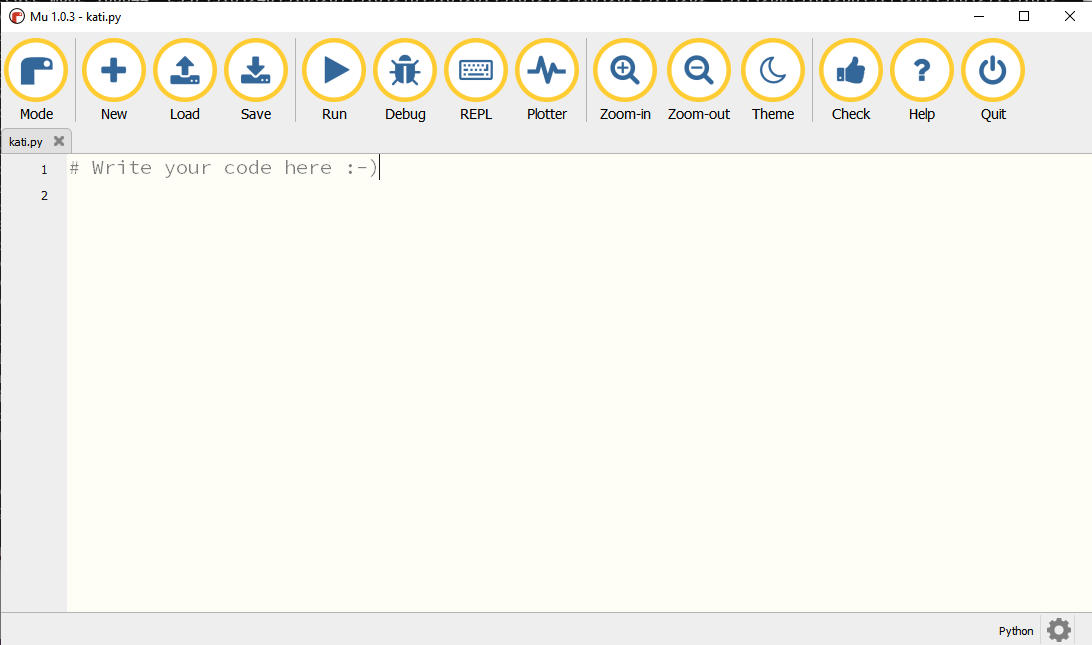
\includegraphics[width=\textwidth]{mu.png}
\label{Mu}
\caption{Mu: Ένας επεξεργαστής προγραμμάτων Python}
\end{figure}

Μπορείς να πατήσεις την εκτέλεση (κουμπί Run) και τότε θα δεις ότι το παράθυρο χωρίζεται σε δύο τμήματα (Εικόνα \ref{Mu2}).  Αν θες να δοκιμάσεις ένα ολόκληρο πρόγραμμα μπορείς να το πληκτρολογήσεις στο βασικό παράθυρο (τώρα γράφει `\#Write your code here`). Ενώ αν θες να δοκιμάσεις κάποια εντολή τότε μπορείς να την πληκτρολογήσεις στο κάτω παράθυρο (τώρα γράφει $>>>$).  Το κάτω παράθυρο ονομάζεται REPL, από τα αρχικά των λέξεων Read, Eval, Print, Loop δηλαδή Διάβασε, Εκτέλεσε (την εντολή/έκφραση), Τύπωσε, Επανάλαβε. Το REPL θα διαβάσει την εντολή, θα την εκτελέσει και θα μας δώσει το αποτέλεσμα.

Από εδώ και πέρα όταν βλέπετε στις σημειώσεις τα τρία σύμβολα ``μεγαλύτερο από'' ($>>>$) θα πληκτρολογείτε τις αντίστοιχες εντολές στο κάτω παράθυρο (REPL). Τα μεγαλύτερα προγράμματα που δεν θα έχουν αυτό το σύμβολο θα τα πληκτρολογείτε στο πάνω παράθυρο.

\fbox{
	\parbox{0.8\textwidth}{%
	\textbf{Συμβουλή:} Αν χρησιμοποιείτε την ηλεκτρονική έκδοση αυτών των σημειώσεων, θυμηθείτε να πληκτρολογείτε τις εντολές και να μην τις κάνετε αντιγραφή επικόλληση.
	}
}


Στην αρχή θα δοκιμάσεις κάποια πράγματα στο κάτω παράθυρο, όμως μην ανησυχείς σύντομα θα γράφεις τα δικά σου προγράμματα στο πάνω παράθυρο.

\begin{figure}
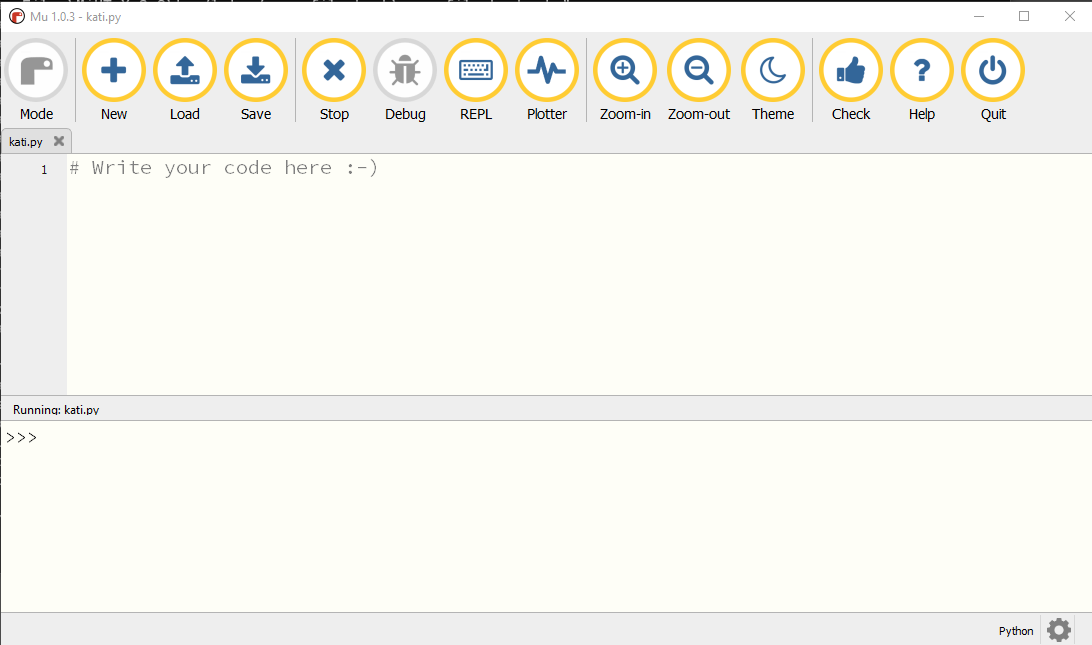
\includegraphics[width=\textwidth]{mu2.png}
\label{Mu2}
\caption{Το πρόγραμμα Mu όταν εκτελείτε ένας κώδικας}
\end{figure}

\section{Το βιβλίο μαθηματικών της Α΄ Γυμνασίου}
Σε αυτές τις σημειώσεις οι περισσότερες ασκήσεις είναι από το βιβλίο Μαθηματικών της Α΄ Γυμνασίου των Βανδουλάκη, Καλλιγά, Μαρκάκη και Φερεντίνου (Εικόνα \ref{matha}).

\begin{figure}
\centering

\includegraphics[width=0.8\textwidth]{matha.jpg}
\label{matha}
\caption{Το εξώφυλλο του βιβλίου των Μαθηματικών που θα χρησιμοποιήσουμε}
\end{figure}